% Author: Izaak Neutelings (November, 2018)
% page 8 https://archive.org/details/StaticAndDynamicElectricity
% https://tex.stackexchange.com/questions/56353/extract-x-y-coordinate-of-an-arbitrary-point-on-curve-in-tikz
% https://tex.stackexchange.com/questions/412899/tikz-calculate-and-store-the-euclidian-distance-between-two-coordinates

\documentclass[border=3pt,tikz]{standalone}
\usepackage{amsmath} % for \dfrac
\usepackage{physics}
\usepackage{tikz,pgfplots}
\usetikzlibrary{angles,quotes} % for pic (angle labels)
\usetikzlibrary{decorations.markings}
\usetikzlibrary{positioning,calc}
\usetikzlibrary{shapes,intersections} % for path name
\pgfplotsset{compat=1.13}
\tikzset{>=latex} % for LaTeX arrow head
\usepackage{xcolor}
\colorlet{Ecol}{orange!90!black}
\colorlet{EcolFL}{orange!80!black}
\colorlet{veccol}{green!45!black}
\colorlet{EFcol}{red!60!black}
\colorlet{pluscol}{red!60!black}
\colorlet{minuscol}{blue!60!black}
\tikzstyle{charged}=[top color=blue!20,bottom color=blue!40,middle color=blue!30,shading angle=10]
\tikzstyle{darkcharged}=[very thin,top color=blue!60,bottom color=blue!80,shading angle=10]
\tikzstyle{gauss surf}=[blue!90!black,top color=blue!2,bottom color=blue!80!black!70,shading angle=5,fill opacity=0.1]
\tikzstyle{gauss line}=[blue!90!black]
\tikzstyle{vector}=[->,thick,veccol]
\tikzstyle{EField}=[->,thick,Ecol]
\tikzset{
  EFieldLine/.style={thick,EcolFL,decoration={markings,
                     mark=at position #1 with {\arrow{latex}}},
                     postaction={decorate}},
  EFieldLine/.default=0.5}
\tikzstyle{measure}=[fill=white,midway,outer sep=2]
\tikzstyle{metal}=[top color=black!10,bottom color=black!20,middle color=black!5,shading angle=35]
\def\L{2.2}
\def\H{2.2}
\def\offset{2.0}
\def\W{0.30}
\def\Nx{5}
\def\Ny{5}


\begin{document}


% BODY charge distribution
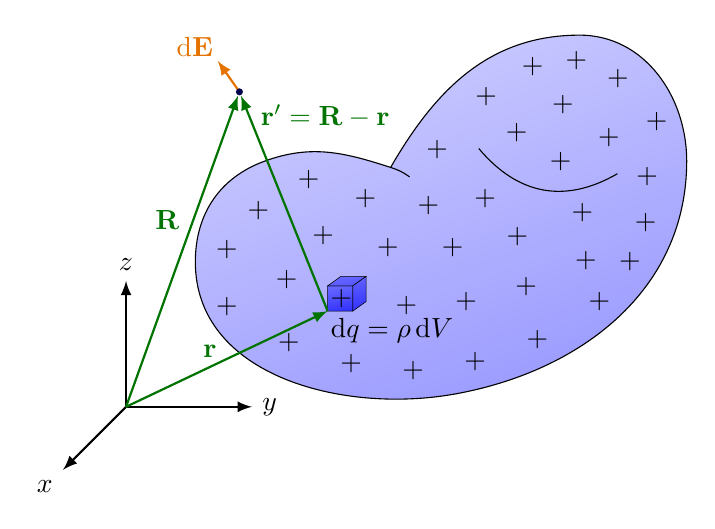
\begin{tikzpicture}[scale=0.8] %[x={(1,0)},y={(0.5,1)}]%,z={(0.73cm,0.73cm)}
  \def\H{3}
  \def\W{5.8}
  \def\h{0.35}
  \def\w{0.42}
  \coordinate (O)  at (-1.1,-0.4);
  \coordinate (P)  at ( 0.7, 4.6);
  \coordinate (Q)  at ( 2.1, 1.12);
  \coordinate (B)  at ( 4.1,-0.2);
  \coordinate (L)  at ( 0.0, 1.9);
  \coordinate (TL) at ( 1.1, 3.5);
  \coordinate (TM) at ( 3.1, 3.4);
  \coordinate (T)  at ( 6.1, 5.5);
  \coordinate (R)  at ( 7.8, 3.5);
  \coordinate (SL) at ( 4.5, 3.7);
  \coordinate (SR) at ( 6.7, 3.3);
  
  % BODY
  \draw[charged,shading angle=20]
    (B) to[out= 10,in=-90] (R)  to[out= 90,in= 0] (T) to[out=180,in= 60] (TM)
        to[out=162,in= 20] (TL) to[out=200,in=90] (L) to[out=-90,in=190] cycle;
  \draw[line width=0.4]
    (TM) to[out=162-180,in=144] ++(0.3,-0.15);
  \draw[line width=0.4] % "smiley"
    (SL) to[out=-50,in=-150,looseness=1.1] (SR);
  
  % CHARGE SIGNS
  \def\Nx{7}
  \def\xmin{0.5}
  \def\xmax{7.4}
  \foreach \i [evaluate={\x=\xmin+(\i-1)*(\xmax-\xmin)/\Nx; \y=0.18+0.12*(\x-3.4)^2;}] in {1,...,\Nx}{
    \node at (\x,\y) {$+$};
  }
  \def\Nx{8}
  \def\xmin{0.5}
  \def\xmax{8.1}
  \foreach \i [evaluate={\x=\xmin+(\i-1)*(\xmax-\xmin)/\Nx; \y=1.2+0.10*(\x-3.5)^2;}] in {1,...,\Nx}{
    \node at (\x,\y) {$+$};
  }
  \def\Nx{7}
  \def\xmin{1.0}
  \def\xmax{8.2}
  \foreach \i [evaluate={\x=\xmin+(\i-1)*(\xmax-\xmin)/\Nx; \y=2.1+0.09*(\x-3.6)^2;}] in {1,...,\Nx}{
    \node at (\x,\y) {$+$};
  }
  \def\Nx{6}
  \def\xmin{4.0}
  \def\xmax{8.1}
  \begin{scope}[rotate around={-6:(6.0,5.1)}]
    \foreach \i [evaluate={\x=\xmin+(\i-1)*(\xmax-\xmin)/\Nx; \y=5.1-0.41*(\x-6.0)^2;}] in {1,...,\Nx}{
      \node at (\x,\y) {$+$};
    }
  \end{scope}
  \def\Nx{3}
  \def\xmin{5.1}
  \def\xmax{7.3}
  \foreach \i [evaluate={\x=\xmin+(\i-1)*(\xmax-\xmin)/\Nx; \y=4.4-0.90*(\x-5.8)^2;}] in {1,...,\Nx}{
    \node at (\x,\y) {$+$};
  }
  %\node at (0.5,1.8) {$+$};
  \node at (1.8,3.2) {$+$};
  \node at (2.7,2.9) {$+$};
  \node at (3.7,2.8) {$+$};
  \node at (4.6,2.9) {$+$};
  \node at (5.8,3.5) {$+$};
  \node at (6.9,1.9) {$+$};
  
  % AXES
  \draw[->,thick] (O) --++ (-1.0,-1.0) node[below left] {$x$};
  \draw[->,thick] (O) --++ ( 2.0, 0.0) node[right] {$y$};
  \draw[->,thick] (O) --++ ( 0.0, 2.0) node[above] {$z$};
  
  % VECTOR dq
  \draw[vector] (O) -- (Q) node[midway,above=0.1,anchor=0] {$\vb{r}$};
  \draw[darkcharged] (Q) |-++ (0.4,0.4) |- cycle;
  \draw[darkcharged] (Q) ++ (0,0.4) --++ (0.21,0.15) --++ (0.4,0) --++ (-0.21,-0.15) -- cycle;
  \draw[darkcharged] (Q) ++ (0.4,0) --++ (0.21,0.15) --++ (0,0.4)
                     node[midway,below=0.25,anchor=140] {$\dd{q}=\rho\dd{V}$} --++ (-0.21,-0.15) -- cycle;
  \node[above right=-0.12] at (Q) {$+$};
  
  % VECTORS
  \draw[EField] (P) --++ (125:0.6) node[above left=-0.1] {$\dd{\vb{E}}$};
  \node[fill=blue!30!black,circle,inner sep=0.9] (P') at (P) {};
  \draw[vector] (Q) -- (P') node[below right=0.2,anchor=170] {$\vb{r}'=\vb{R}-\vb{r}$};
  \draw[vector] (O) -- (P') node[midway,above left=0.2,anchor=-80] {$\vb{R}$};
  
  % DEBUG
  %\node at (B) {B};
  %\node at (L) {L};
  
\end{tikzpicture}


% BODY
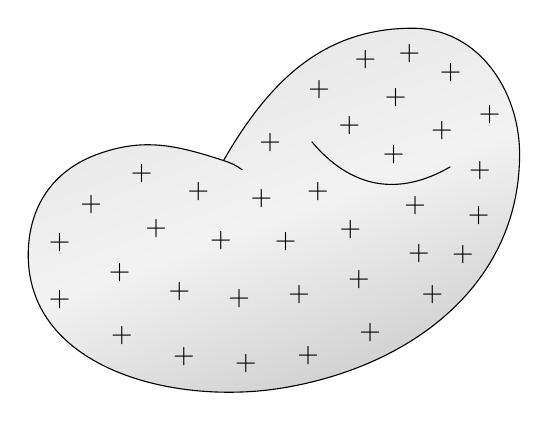
\begin{tikzpicture}[scale=0.8] %[x={(1,0)},y={(0.5,1)}]%,z={(0.73cm,0.73cm)}
  \def\H{3}
  \def\W{5.8}
  \def\h{0.35}
  \def\w{0.42}
  \coordinate (O)  at (-1.1,-0.4);
  \coordinate (P)  at ( 0.7, 4.6);
  \coordinate (Q)  at ( 2.29, 1.34);
  \coordinate (B)  at ( 4.1,-0.2);
  \coordinate (L)  at ( 0.0, 1.9);
  \coordinate (TL) at ( 1.1, 3.5);
  \coordinate (TM) at ( 3.1, 3.4);
  \coordinate (T)  at ( 6.1, 5.5);
  \coordinate (R)  at ( 7.8, 3.5);
  \coordinate (SL) at ( 4.5, 3.7);
  \coordinate (SR) at ( 6.7, 3.3);
  
  % BODY
  \draw[metal,shading angle=20]
    (B) to[out= 10,in=-90] (R)  to[out= 90,in= 0] (T) to[out=180,in= 60] (TM)
        to[out=162,in= 20] (TL) to[out=200,in=90] (L) to[out=-90,in=190] cycle;
  \draw[line width=0.4]
    (TM) to[out=162-180,in=144] ++(0.3,-0.15);
  \draw[line width=0.4] % "smiley"
    (SL) to[out=-50,in=-150,looseness=1.1] (SR);
  
  % CHARGE SIGNS
  \def\Nx{7}
  \def\xmin{0.5}
  \def\xmax{7.4}
  \foreach \i [evaluate={\x=\xmin+(\i-1)*(\xmax-\xmin)/\Nx; \y=0.18+0.12*(\x-3.4)^2;}] in {1,...,\Nx}{
    \node at (\x,\y) {$+$};
  }
  \def\Nx{8}
  \def\xmin{0.5}
  \def\xmax{8.1}
  \foreach \i [evaluate={\x=\xmin+(\i-1)*(\xmax-\xmin)/\Nx; \y=1.2+0.10*(\x-3.5)^2;}] in {1,...,\Nx}{
    \node at (\x,\y) {$+$};
  }
  \def\Nx{7}
  \def\xmin{1.0}
  \def\xmax{8.2}
  \foreach \i [evaluate={\x=\xmin+(\i-1)*(\xmax-\xmin)/\Nx; \y=2.1+0.09*(\x-3.6)^2;}] in {1,...,\Nx}{
    \node at (\x,\y) {$+$};
  }
  \def\Nx{6}
  \def\xmin{4.0}
  \def\xmax{8.1}
  \begin{scope}[rotate around={-6:(6.0,5.1)}]
    \foreach \i [evaluate={\x=\xmin+(\i-1)*(\xmax-\xmin)/\Nx; \y=5.1-0.41*(\x-6.0)^2;}] in {1,...,\Nx}{
      \node at (\x,\y) {$+$};
    }
  \end{scope}
  \def\Nx{3}
  \def\xmin{5.1}
  \def\xmax{7.3}
  \foreach \i [evaluate={\x=\xmin+(\i-1)*(\xmax-\xmin)/\Nx; \y=4.4-0.90*(\x-5.8)^2;}] in {1,...,\Nx}{
    \node at (\x,\y) {$+$};
  }
  %\node at (0.5,1.8) {$+$};
  \node at (1.8,3.2) {$+$};
  \node at (2.7,2.9) {$+$};
  \node at (3.7,2.8) {$+$};
  \node at (4.6,2.9) {$+$};
  \node at (5.8,3.5) {$+$};
  \node at (6.9,1.9) {$+$};
  
\end{tikzpicture}


% BODY
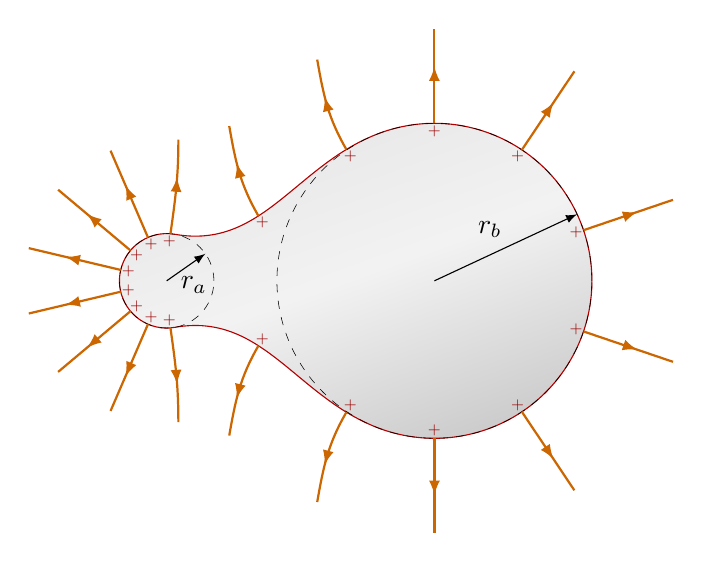
\begin{tikzpicture}
  \def\C{3.4}
  \def\Ra{0.6}
  \def\Rb{2.0}
  \def\q{0.1}
  \def\E{1.2}
  \def\anga{80}
  \def\angb{110}
  \def\Na{3}
  \def\Nb{2}
  \def\Nc{4}
  \coordinate (C1)  at (0,0);
  \coordinate (C2)  at (\C,0);
  \coordinate (T) at ({\C+\Rb*cos(\angb)},{\Rb*sin(\angb)});
  
  % BODY
  \draw[metal,shading angle=20,red!70!black,name path=body]
    (-\anga:\Ra) arc(-\anga:-360+\anga:\Ra) to[out=\anga-90,in=\angb+90]
    (T) arc( \angb:-\angb:\Rb) to[out=-\angb-90,in=90-\anga] cycle;
  \draw[dashed,line width=0.2]
    (C1) circle (\Ra);
  \draw[dashed,line width=0.2]
    (C2) circle (\Rb);
  \draw[->] (C1) --++ (35:\Ra) node[midway,right=0.1,below] {$r_a$};
  \draw[->] (C2) --++ (25:\Rb) node[midway,left=0.2,above] {$r_b$};
  
%  % CHARGE SIGNS
%  \foreach \i [evaluate={\x=\xmin+(\i-1)*(\xmax-\xmin)/\Nx; \y=0.18+0.12*(\x-3.4)^2;}] in {1,...,\Nx}{
%    \node at (\x,\y) {$+$};
%  }
  
  % ELECTRIC FIELD
  \foreach \i [evaluate={\ang=(\i-0.5)*80/\Na;}] in {1,...,\Na}{
    \draw[EFieldLine={0.6}]
      (C1)++( 180-\ang:\Ra) --++ ( 180-\ang:\E);
    \draw[EFieldLine={0.6}]
      (C1)++(-180+\ang:\Ra) --++ (-180+\ang:\E);
    \node[pluscol,scale=0.6] at ( 180-\ang:\Ra-\q) {$+$};
    \node[pluscol,scale=0.6] at (-180+\ang:\Ra-\q) {$+$};
  }
  \foreach \i [evaluate={\ang=(\i-0.5)*75/\Nb;}] in {1,...,\Nb}{
    \draw[EFieldLine={0.6}] (C2)++( \ang:\Rb) --++ ( \ang:\E);
    \draw[EFieldLine={0.6}] (C2)++(-\ang:\Rb) --++ (-\ang:\E);
    \node[pluscol,scale=0.6] at ($(C2)+( \ang:\Rb-\q)$) {$+$};
    \node[pluscol,scale=0.6] at ($(C2)+(-\ang:\Rb-\q)$) {$+$};
  }
  \foreach \i [evaluate={\x=0.08*\Ra+(\i-1)*(\C-0.08*\Ra)/(\Nc-1);}] in {1,...,\Nc}{ % intersections
    \path[name path global/.expanded=ETline\i] (\x,0) --++ (90:1.1*\Rb);
    \path[name path global/.expanded=EBline\i] (\x,0) --++ (-90:1.1*\Rb);
  }
  \foreach \i/\ang/\in in {1/82/-90,2/120/-80,3/120/-80,4/90/-90}{
    \draw[EFieldLine={0.6},name intersections={of=body and ETline\i,name=ET\i}]
      (ET\i-1) to[out=\ang,in=\in]++ ({90+0.6*(\ang-90)}:\E);
    \draw[EFieldLine={0.6},name intersections={of=body and EBline\i,name=EB\i}]
      (EB\i-1) to[out=-\ang,in=-\in]++ ({-90-0.6*(\ang-90)}:\E);
    \node[pluscol,scale=0.6] at ($(ET\i-1)+( \ang+180:\q)$) {$+$};
    \node[pluscol,scale=0.6] at ($(EB\i-1)+(-\ang-180:\q)$) {$+$};
  }
  
\end{tikzpicture}


\end{document}
